\chapter{AD-HOC, DECENTRALIZED GRIDS}
\label{chap:gridappliance}

``Give a man a fish, feed him for a day.  Teach a man to fish, feed him for a
lifetime'' -- Lau Tzu

Large-scale grid computing projects such as TeraGrid and Open Science Grid
provide researchers vast amounts of compute resources but with requirements
that could limit access, results delayed due to potentially long job queues,
and environments and policies that might affect a user's work flow. In many
scenarios and in particular with the advent of Infrastructure as a Service
(IaaS) cloud computing, individual users and communities can benefit from less
restrictive, dynamic systems that include a combination of local resources and
on-demand resources provisioned by one or more IaaS provider.  These types of
scenarios benefit from flexibility in deploying resources, remote access, and
environment configuration.

Grid computing presents opportunities to combine distributed resources to form
powerful systems.  Due to the challenges in coordinating resource configuration
and deployment, researchers tend to either become members of existing grids or
deploy their own private resources.  The former approach is limited by lack of
flexibility in the environment and policies, while the latter requires
expertise in systems configuration and management.  Though there exists a
wealth of middleware available, including resource managers such as
Condor~\cite{condor0}, Torque (PBS)~\cite{torque}, and Sun Grid
Engine~\cite{grid_engine}, many see the cost of installing and managing these
systems as being greater than their usefulness and as a result turn to
inefficient ad hoc resource discovery and allocation.  To combine resources
across multiple domains solutions there exist solutions such as the Globus
Toolkit~\cite{globus} or gLite~\cite{glite}; however, these tool sets come with
their own challenges that require the level of expertise most researchers in
fields outside of information technology lack.

With the recent advent of cost-effective on-demand computing through
Infrastructure as a Service ``clouds'', new opportunities for user-deployed
grids have arisen; where, for example, a small local computer cluster can be
complemented by dynamically provisioned resources that run ``cloud-burst''
workloads.  However, while cloud-provisioned resources solve the problem of
on-demand instantiation, the problem of how to {\em configure} these resources
to seamlessly and securely integrate with one's infrastructure remains a
challenge.  In particular, considering that users may provision resources from
multiple IaaS providers, the configuration demands are similar to a distributed
grid: while a cloud image can be encapsulated with a grid computing stack, it
still needs configuration in terms of allocating and distributing the
appropriate certificates, network configuration to establish end-to-end
connectivity, and proper configuration of the middleware to establish worker,
submit, and scheduler nodes.  

In this chapter, I present techniques that reduce the entry barrier in terms of
necessary expertise and time investment in deploying and extending ad hoc,
distributed grids.  To verify this assertion, I have implemented a system
supporting these ideas in the ``Grid Appliance,'' which as will be
demonstrated, allows users to focus on making use of a grid while minimizing
their efforts in setting up and managing the underlying components.  The core
challenges solved by my approach include:

\begin{itemize}
\item decentralized directory service for organizing grids,
\item decentralized job submission,
\item grid single sign on through web services and interfaces,
\item sandboxing with network support,
\item and all-to-all connectivity despite network asymmetries.
\end{itemize}

\begin{figure}
\centering
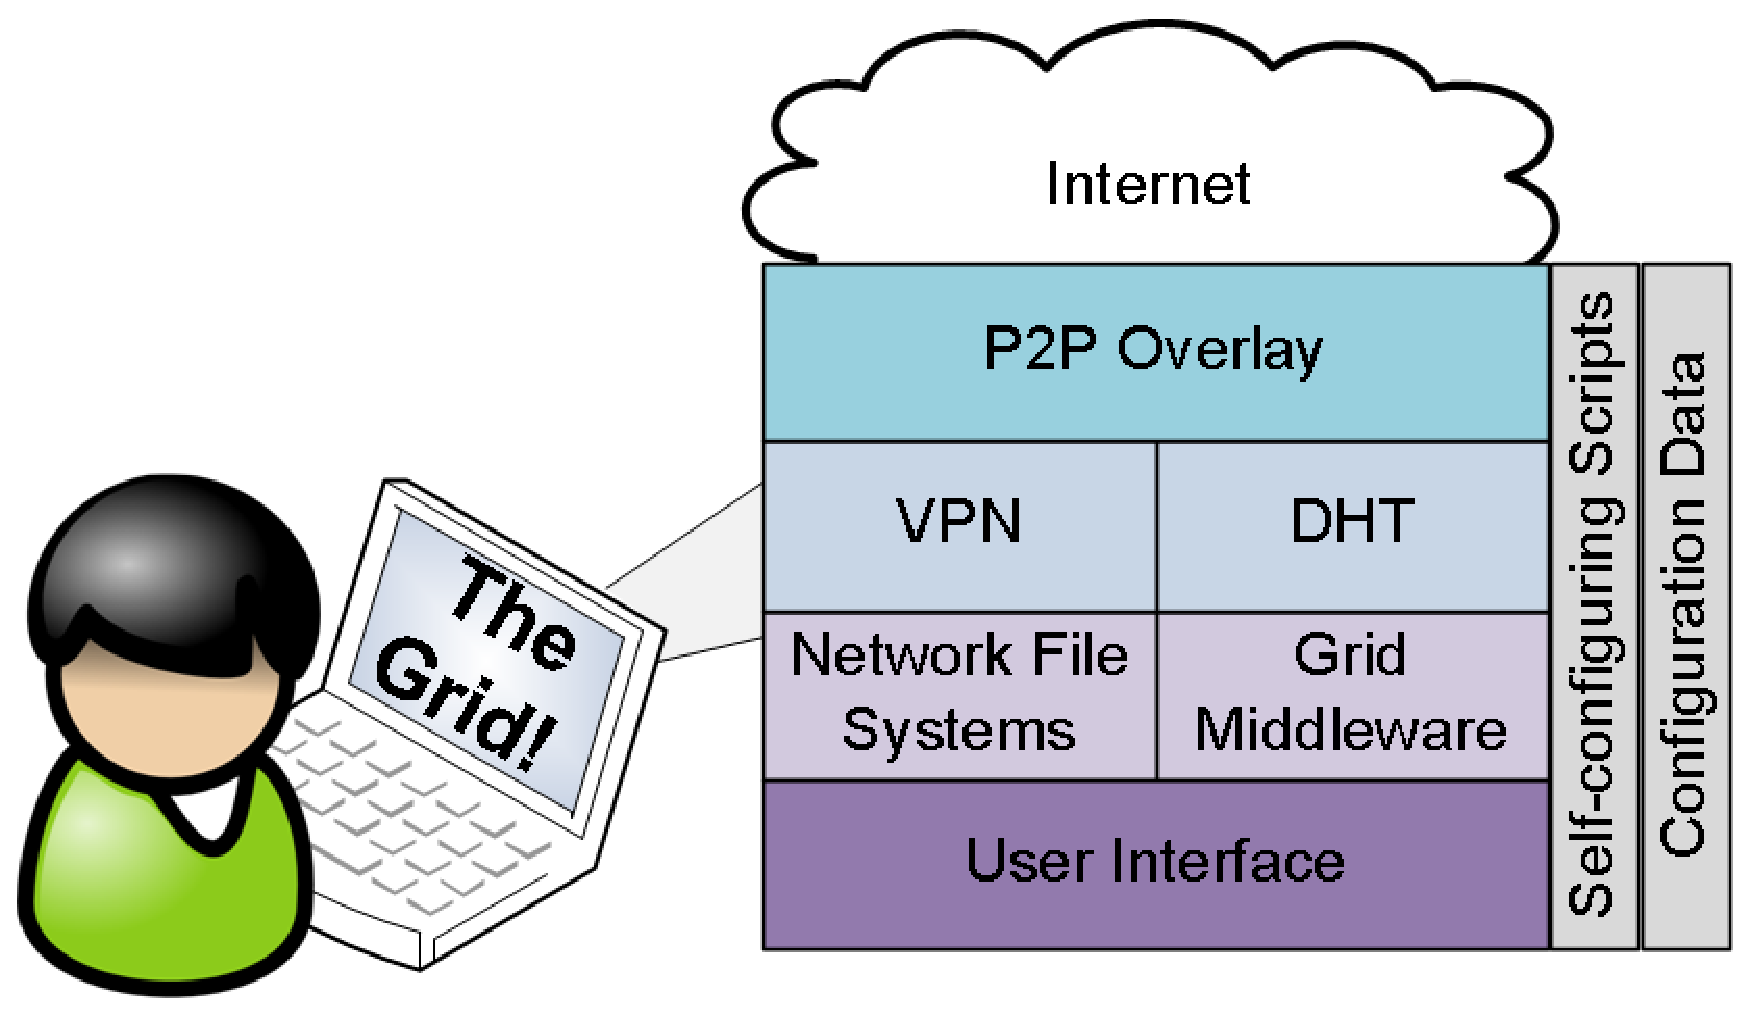
\includegraphics[width=4in]{figs/appliance_overlays.eps}
\caption{Grid Appliance middleware}
\label{fig:appliance}
\end{figure}

The ``Grid Appliance'' project and concepts have been actively developed and
used in several projects for the past six years.  Of these projects, Archer, a
distributed grid for computer architecture research,
has demonstrated the feasibility and utility of this approach by
deploying a shared collaborative infrastructure spanning clusters across six US
universities, where the majority of the nodes are constrained by network
address translation (NAT).  Every resource in Archer is configured in the same,
simple manner:  by deploying a ``Grid Appliance'' that self-configures to join a
wide-area grid.  Researchers interested or desiring the ability to access both
grid resources and specialized commercial simulation tools (such as Simics) can
easily use and contribute resources from this shared pool with little effort
by joining a website, downloading a configuration image and a virtual
machine (VM), and starting the VM inside a VM manager (VMM).  Upon completion of
the booting process, users are connected to the grid and able to submit and
receive jobs.

At the heart of my approach lies a P2P (peer-to-peer) infrastructure based upon
a distributed hash table (DHT) useful for decentralized configuration and
organization of systems.  Peers are able to store key, value pairs into the DHT
and to query the DHT with a key and potentially receive multiple values
efficiently.  The DHT provides discovery and coordination primitives for the
configuration of a decentralized P2P virtual private network (VPN), which
supports unmodified applications across a network overlay.  The DHT is also
used for the decentralized coordination of the grid.  Users can configure their
grid through a web interface, which outputs configuration files that can be
used with the ``Grid Appliance.''

The techniques described in this paper have many applications.  The basic
system supports the creation of local grids by starting a virtual machine on
the computers intended for use within the grid and using LAN multicast for
discovery.  It allows users to seamlessly combine their dedicated grids with
external resources such as workstations and cloud resources.  The level of
familiarity with security, operating systems, and networking is minimal as all
the configuration details are handled as components of the system.  Management
of the system including users and network configuration utilizes a social
networking like group interface, while deployment uses pre-built virtual
machine images.  A graphical overview of the system is illustrated in
Figure~\ref{fig:appliance}.

These techniques simplify the tethering of resources across disparate networks
The setup of security, connectivity, and their continuous management imposes
considerable administrative overhead, in particular when networks are
constrained by firewalls and NAT devices that prevent direct communication with
each other, and which are typically outside the control of a user or lab.  Our
approach integrates decentralized systems behind NATs in a manner that does not
require the setup of exceptions and configuration at NAT/firewall by system
administrators.

The rest of the paper is as follows.  Section~\ref{wow} highlights of my
research groups previous work to provide background for my contributions in
this paper.  In Section~\ref{architecture}, I describe the components of the
``Grid Appliance'' WOW.  Section~\ref{case_study} provides a case study of a
grid deployment using standard grid deployment techniques compared to our
``Grid Appliance,'' describing qualitatively the benefits and evaluating
quantitatively the overheads of this approach.  I share my experiences from
this long running project in Section~\ref{lessons_learned}.  Finally,
Section~\ref{related_work} compares and contrasts other solutions to these
problems.

\section{WOWs}
\label{wow}

This work furthers the vision began by myself and my research lab in earlier
described as work wide-area overlay of virtual workstations~\cite{wow} (WOW).
The WOW paper established the use of virtualization technologies, primarily
virtual networking and virtual machines, to support dynamic allocation of
additional resources in grids that span wide area networks.  For reference, the
extensions made in this paper to the WOW concept are means for the dynamic
creation of grids with support for security, decentralized access, and
user-friendly approaches to grid management.  This section covers the
development of WOWs over the years as it relates to other publications and as
means to distinguish the contributions made by me and in this chapter.

\subsection{P2P Overlays}

Peer-to-peer or P2P systems create environments where members have a common
functionality.  P2P systems are often used for discovery in addition to some
user-specific service, such as voice and video with Skype$^\registered$ or data sharing with
BitTorrent$^\registered$.  Many forms of P2P have autonomic features such as self-healing and
self-optimization with the ability to support decentralized environments.  As I
will show, this makes their application in the system very attractive.

For the ``Grid Appliance,'' I have chosen to use Brunet~\cite{brunet}, a type of
structured overlay.  Structured overlays tend to be used to construct
distributed hash tables (DHT) and in comparison to unstructured overlays
provide faster guaranteed search times ($O(\log N)$ compared to $O(N)$, where N
is the size of the network).  The two most successful structured overlays are
Kademlia~\cite{kademlia}, commonly used for decentralized BitTorrent$^\registered$, and
Dynamo~\cite{dynamo}, to support Amazon$^\registered$'s web site and services.

Brunet support for NAT traversal makes it unique from other structured
overlays.  Originally in the WOWs~\cite{wow}, Brunet facilitated the dynamic
connections amongst peers in the grid.  Since then, it has been extended to
support DHT with atomic operations~\cite{pcgrid07}, efficient relays when
direct NAT traversal fails~\cite{groupvpn}, resilient overlay structure and
routing~\cite{hpdc08_0}, and cryptographically secure
messaging~\cite{groupvpn}.

\subsection{Virtual Private Networks}

A common question with regards to this work is ``why VPNs?''  The core reason
is connectivity.  IPv4 (Internet Protocol version 4) has a limited address
space, which has been extended through the use of NAT allowing a single IP to
be multiplexed by multiple devices.  This creates a problem; however, as it
breaks symmetry in the Internet limiting the ability for certain peers to
become connected and which peers can initiate connections.  With the advent of
IPv6 (Internet Protocol version 6), the situation might improve, but there are
no guarantees that NATs will disappear nor can users be certain that firewalls
will not be in place that inhibit symmetry.  A VPN circumvents these issues, so
long as the user can connect to the VPN, as all traffic is routed through a
successfully connected pathway.

The problem with traditional VPN approaches is management overhead including
maintaining resources on public IP addresses and establishing links amongst
members in the VPN.  The VPN used in the system is called IPOP~\cite{groupvpn,
ipop}.  IPOP (IP over P2P), as the name implies, uses a P2P overlay (Brunet) to
route IP messages.  By using P2P, maintaining dedicated bootstrap nodes have
less overhead, my approach with IPOP allows an existing Brunet infrastructure
to bootstrap independent Brunet infrastructures in order to isolate IPOP
networks in their own environments~\cite{bootstrapping}.

Once IPOP has entered its unique Brunet overlay, it obtains an IP address.  IP
address reservation and discovery relies on Brunet's DHT.  Each VPN stores its
P2P identifier into the DHT at the generated by the desired IP address, such
that the key, value pair is $(hash(IP), P2P)$.  In order to ensure there are no
conflicts, the storing of this value into the DHT uses an atomic operation,
which succeeds only if no other peer has stored a value int $hash(IP)$.

The process for creating connections begins when IPOP receives an outgoing
message.  First it parses the destination address and queries the DHT for the
remote peers P2P address.  The peer then attempts to form a secure, direct
connection with the remote peer using Brunet's secure messaging layer.  Once
that has formed, packets to that IP address are directed over that secure link.

In my original design~\cite{vtdc}, the virtual network was secured through a
kernel-level IPsec stack, a model kept through the first generation Archer
deployment.  This approach only secures virtual network links between parties
and does not secure the P2P layer; furthermore, in IPsec configuration each
peer requires a unique rule for every other peer, which limited the maximum
number of peers in the VPN.  Securing the P2P layer is important, otherwise
malicious users could easily derail the entire system, but securing with IPsec
would practically negate the benefits of the P2P system, because of network
configuration issues related to NATs and firewalls.  In modern deployments, I
have employed the security layer at the P2P layer, which in turn also secures
virtual networking links.

For grids that rely upon VPNs to connect resources and users, this can impose
the need for a certificate for the VPN and one for the grid.  Though in our
approach, I avoid this problem by using a VPN that allows a user to verify the
identity of a remote peer and obtain its certificate, and have taken advantage
of hooks in grid software that are called to verify a remote peers
authenticity.  In other words, user access is limited by the VPN and identity
inside the grid is maintained by that same certificate.  This might not be
possible if all users were submitting from the same resources but is feasible
in the system since each user submits from their own system.

\subsection{Virtual Machines in Grid Computing}

Earlier work~\cite{fig_grid} advocated the use of virtual machines (VMs) in
grid computing for improved security and customization.  Others
since~\cite{sandbox, dve, ourgrid_paper} have been established VMs as means for
sandboxing, that is environments that allow untrusted users to use trusted
resources in a limited fashion.  VMs run as a process on a system, where
processes running inside the VM have no access to the host operating system.
Furthermore, VMs can have limited or no networking access as controlled by the
host, which effectively seals them in a cage or sandbox protecting the hosts
environment.  VMs are also useful for customization and legacy applications,
since a developer can configure the VM and then distribute it as an appliance,
with the only requirement on the end user being that they have a VM software or
manager.  Quantitatively, previous work has shown that CPU-bound tasks perform
fairly well running with no more than 10\% overhead and in some cases 0\%,
which is the case with VMs like Xen.

While not a direct correlation to grid computing, clouds have benefited
significantly from VMs.  VMs are the magic behind cloud infrastructures that
provide IaaS, such as EC2.  In these environments, users are able to create
customized instances, or packaged operating systems and applications, inside of
cloud environments, share with each other, and dynamically create or shutdown
them as necessary.  While the application of clouds is generic, it can easily
be applied towards grids.  A user can create push excess jobs into the cloud,
when there is overflow, high demands, or the user does not want to maintain
their own hardware.  One challenge, however, is the dynamic creation of a grid
as well as extension of an existing grid using the cloud, challenges that are
addressed in this paper.

\section{Architectural Overview}
\label{architecture}

My approach attempts to reuse as many available components to design a grid
middleware generic enough that th ideas can be applied to other middleware
stacks.  As a result, my contribution in this chapter and in particular this
section focuses primarily on the following key tasks:  making grid construction
easy, supporting decentralized user access, sandboxing the users environment,
limiting access to the grid to authorized identities, and ensuring priority on
users own resources.  

\begin{center}
\begin{table}
\caption{Grid middleware comparison}
\footnotesize{
\begin{tabular}[c]{p{1.6cm}p{3.25cm}p{3.4cm}p{3.2cm}p{3.05cm}} \hline
& Description & Scalability & Job queue / submission site & API Requirements \\ \hline
Boinc &
Volunteer computing, applications ship with Boinc and poll head node for data
sets &
Not explicitly mentioned, limited by the ability of the scheduler to handle
the demands of the client &
Each application has a different site, no separation from job queue and
submission site &
Boinc API and middleware bundling required
\\
BonjourGrid &
Desktop grid, use zeroconf / Bonjour to find available resources in a LAN &
No bounds tested, limits include multicasting overheads and processing power
of job queue node &
Each user has their own job queue / submission site &
None \\
Condor &
High throughput computing / on demand / desktop / etc / general grid computing &
Over 10,000$^{1}$ &
Global job queue, no limit on submission sites, submission site communicates directly with worker nodes &
Optional API to support job migration and check pointing \\
PastryGrid &
Use structured overlay Pastry to form decentralized grids &
Decentralized, single node limited by its processing power, though
collectively limited by the Pastry DHT &
Each connected peer maintains its own job queue and submission site &
None \\
PBS / Torque~\cite{torque} &
Traditional approach to dedicated grid computing &
up to 20,000 CPUs$^{2}$ &
Global job queue and submission site &
None
\\
SGE &
Traditional approach to dedicated grid computing &
Tested up to 63,000 cores on almost 4,000 hosts$^{3}$ &
Global job queue and submission site &
None
\\
XtremWeb &
Desktop grid, similar to Condor but uses pull instead of push, like Boinc &
Not explicitly mentioned, limited by the ability of the scheduler to handle
the demands of clients &
Global job queue, separate submission site, optionally one per user &
No built-in support for shared file systems
\\ \hline
\end{tabular}
}
\label{tab:grid}
\end{table}
\end{center}

\addtocounter{footnote}{1}
\footnotetext[\value{footnote}]{\url{http://www.cs.wisc.edu/condor/CondorWeek2009/condor\_presentations/sfiligoi-Condor\_WAN\_scalability.pdf}}
\addtocounter{footnote}{1}
\footnotetext[\value{footnote}]{\url{http://www.clusterresources.com/docs/211}}
\addtocounter{footnote}{1}
\footnotetext[\value{footnote}]{\url{http://www.sun.com/offers/docs/Extreme\_Scalability\_SGE.pdf}}

\subsection{Web Interface and the Community}

Before deploying any software or configuring any hardware, a grid needs
organization including certificate management, grid access, user account
management, and delegation of responsibilities.  These are complex questions,
which can be challenging to address, though for less restrictive systems, like
a collection of academic labs sharing clusters, they may be very easy.  One of
the professors could handle the initial authorization of all the other labs and
then delegate to them the responsibility of allowing their affiliates, such as
students and scholars access.

For academic environments, grids become more challenging when the professor or
worse yet students must maintain the certificates, handling certificate
requests, and placing signed certificates in the correct location.  Our
solution to this potentially confusing area was a group interface, akin to
something like Facebook$^\registered$'s or Google$^\registered$'s groups.  Albeit, those types of groups
are not hierarchal, which is a necessity in order to have delegated
responsibilities.  Thus I have a two layer approach, a grid group for members
of the grid trusted by the grid organizers and user groups for those who are
trusted by those in the grid group.  Members of the grid group can create their
own user groups.  A member of a user group can gain access to the grid by
downloading grid configuration data available within the user group web
interface.  This configuration data comes in the format of a disk image, when
added to a ``Grid Appliance'' VM, it is used to obtain the user's credentials
and enabling them to connect to the grid.

To give an example, consider the computer architecture grid, Archer.  Archer
was seeded initially by the University of Florida, so my group and I are the
founders and maintainers of the Archer grid group.  As new universities and
independent researchers have joined Archer, they request access to this group.
Upon receiving approval, they then need to form their own user group so that
they can allow others to connect to the grid.  So a trusted member might create
a user group titled ``Archer for University X'' and all members of university X
will apply for membership in that group.  The creator can make decisions to
either accept or deny these users.  Once the user has access, they will
download their configuration data formatted as a virtual disk image and the
``Grid Appliance'' VM and start the ``VM.''  After starting the VM, the user
will be connected to the grid and able to submit and receive jobs.

\begin{figure}
\centering
\epsfig{file=figs/system.eps, width=\textwidth}
\caption{Grid Appliance deployment scenario}
\label{fig:system}
\end{figure}

Joining is easy; a grid requires a user to sign onto a website and download a
configuration data, which can then be used on multiple systems.  To support
this process, the configuration data contains cryptographic information that
facilitates acquisition of a signed certificate from the web interface through
XML-RPC over HTTPS (Extensible Markup Language Remote Procedure Call over
Hypertext Transfer Protocol Secure).  The process begins by either booting the
``Grid Appliance'' or restarting a ``Grid Appliance'' service.  When starting
the service will detect if there is new configuration data, and if there is, it
contacts the web interface with the cryptographic information and a public key.
The web interface verifies the user's identity, retrieves their profile from
its database and binds that information with the public key to create a
certificate request, which will then be signed and returned to the user.

With a public web interface, I have been able to create a variety communities.
One of particular interest is not the grid itself but rather a bootstrapping
community for grids.  The web interface has been designed to support many grid
groups, so too has the P2P infrastructure as it supports bootstrapping into
unique private overlays for individual grids by means of Brunet's ability to
support recursive bootstrapping.  By using the public interface, users have an
opportunity to reuse a public bootstrap infrastructure and only need to focus
on the configuration of their VPN and grid services, which has been trivialized
to accepting or denying users access to a group and turning on resources.  We
would like to note that there is no need to make an explicit public grid
community through the web interface, since all ``Grid Appliances'' come with a
default configuration file that will connect them to an insecure public grid.  

\subsection{The Organization of the Grid}

The previous section focused facilitation of grid configuration using the web
interface and skirted the issues of detailed configuration and organization.
The configuration of the grid mirrors that of the connection process.  The
first tier group maps to a common grid and each grid maps to a VPN.  Thus when
a user creates a new grid group, they are actually configuring a new VPN, which
involves address range, security parameters, user agreements, and the name of
the group.  The system provides defaults for address range and security
parameters, so users can focus on high level details like the user agreement
and the grid's name.

As mentioned earlier, the second tier of groups enables members in the grid
group to provide access to their community.  It is also the location that users
download their configuration data.  The configuration files come in three
flavors: submission, worker, or manager.  Worker nodes strictly run jobs.
Submission nodes can run jobs as well as submit jobs into the grid.  Manager
nodes are akin to head nodes, those that manage the interaction between worker
and submission nodes.

While the configuration details are handled by the web interface and scripts
inside the ``Grid Appliance,'' organization of the grid, more specifically the
linking of worker and submission nodes to manager nodes, relies on the DHT.
Managers store their IP addresses into the DHT at the key \emph{managers}.
When workers and clients join the grid, they automatically query this key,
using the results to configure their grid software.  Managers can also query
this key to learn of other managers to coordinate with each other.

\subsubsection{Selecting a Middleware}

My grid composition is largely based upon a desire to support a decentralized
environment, while still retaining reliability and limiting documentation
support efforts.  As there exist many middlewares to support job submission and
scheduling, I surveyed available and established middleware to determine how
well they matched my requirements.  My results are presented in
Table~\ref{tab:grid}, which covers most of the well established middleware and
some recent research projects focused on decentralized organization.

Of the resource management middlewares surveyed, I chose to use Condor as it
matches closest with my goals due to its decentralized properties and focus on
desktop grids.  Condor allows multiple submission points, a non-trivial
obstacle in some of the other systems.  Additionally, adding and removing
resources in Condor can be done without any configuration from the managers.
Conversely, in SGE and Torque, after resources have been added into the system,
the administrator must manually configure the manager to control them.  Most
scheduling software assumes that resources are dedicated, while Condor supports
opportunistic cycles, by detecting the presence of other entities and will
suspend, migrate, or terminate a job, thus enabling desktop grids.  A common
drawback to established middlewares is the requirement of a manager node;
having no manager in an ad hoc grid would be ideal.

\subsubsection{Self-Organizing Condor}

While the requirement of a central manager may be undesirable, they can easily
be run inside a VM and Condor supports the ability to run many in parallel
through the use of ``flocking~\cite{flocking}.'' Flocking allows submission
sites to connect to multiple managers.  This serves two purposes: 1) to provide
transparent reliability by supporting multiple managers and 2) users can share
their resources through their own manager.  Flocking allows each site to run
its own manager or share the common manager.  

To configure Condor, manager IP addresses are stored into the DHT using the key
\emph{managers}.  Joining peers query the DHT to obtain a list of managers,
selecting one randomly to use as its primary manager with the result used for
flocking.  If the system prefers managers from its group, it will randomly
contact each manager in an attempt to find a match, selecting one at random if
no match is found.  Until a manager is found, the process repeats every 60
seconds.  Upon finding a manager, the state of the system is verified every 10
minutes and new managers are added to the flock list.

\subsubsection{Putting It All Together}

The following summarizes the configuration and organization of the grid.
Minimally a grid will constitute a manager, some workers, and a submitter.
Referencing Figure~\ref{fig:system} step ``1,'' during system boot, without
user interaction, each machine contacts the group website to obtain a valid VPN
certificate.  Whereupon, it connects to the P2P overlay whose bootstrap peers
are listed inside the configuration file, ``step 2.''  At which point, the
machine starts the VPN service running on top of the P2P overlay, also part of
step ``2.'' The self-configuring VPN creates a transparent layer hiding from
the user and administrators the complexity in setting up a common fabric that
can handle potential network dynamics.  Machines automatically obtain a unique
IP address and find their place inside the grid.  For a manager machine, this
means registering in the DHT (not shown), while clients and workers search for
available managers by querying the DHT, step ``3;'' IPOP translates the IP to a
P2P address, step ``4;'' and then client contacts the manager directly, step
``5.''

\subsection{Sandboxing Resources}

As tasks can run on worker and potentially submission nodes, I have devised
means to sandbox the environments that do not limit user interactions with the
system.  While more traditional approaches to sandboxing emphasize a separation
between worker and submission machine, in actual deployments, very few users
explicitly deploy worker machines, most are submission machines.  Thus I
developed sandboxing techniques to limit the ability of submitted jobs on
systems that are simultaneously being used for submission.  So these sandboxing
technique considers more than just locking down the machine but also ensuring a
reasonable level of access.

\subsubsection{Securing the Resources}

The core of my sandboxing approach is to limit attacks to software in the
system and not poorly configured user space, such as poorly chosen passwords or
resources external to the ``Grid Appliance.''  All jobs are run as a set of
predefined user identities.  When the jobs are finished executing, whether
forcibly shutdown or completed successfully, all processes from that user are
shutdown, preventing malicious trojan attacks.  Those users only have access to
the working directory for the job and those with permission for everybody.
Escalation of privilege attacks due to poor passwords are prevented by
disallowing use of ``su'' or ``sudo'' for these users.  Finally, network access
is limited to the VPN, thus they are unable to perform denial of service
attacks on the Internet.

Additionally, systems can be configured such that the only network presented to
them is that of the virtual network.  To support this, IPOP has been enhanced to
support a router mode, which can be bridged to a virtual machine adapter
running on the host machine that connects to the network device running inside
the VM.  Not only does this improve performance, due to reduced I/O overhead,
the same virtual network router can be used for multiple VMs.

To ensure that submit machines still have a high level of functionality without
risking the system to external attacks even from users on the same network,
user services are run only on a ``host-only'' network device within the virtual
machine.  This includes an SSH server and a Samba or Windows File Share.  The
user name matches that from the website, while the password defaults to
``password.''  I would like to note that file sharing services work the
opposite to that of host to guest as most VMs already have in place.  Instead
users can access their files on the VM from the host.  This was done to limit
potential attacks on submission machine.

\subsubsection{Respecting the Host}

Another aspect of sandboxing is respecting the usage of the host.  While Condor
can detect host usage on a machine it is running, when run inside a VM it
cannot detect usage on the host.  Thus it is imperative to support such a
configuration otherwise my approach would be limited in that it can only be
run during idle times.  In the ``Grid Appliance'', this is addressed by running
a light-weight agent on the host that communicates to the VM through the second
Ethernet interface.  The agent discovers a VM through multicast service
discovery executed only on "host-only" virtual network devices.  When a user
accesses the host, the agent notifies a service in the VM, which results in
running tasks being suspended, migrated, or terminated.  The machine remains
off limits until there has been no user activity for 10 minutes.

\subsubsection{Decentralized Submission of Jobs}

From the administrator's perspective, not requiring a submission machine is
also a form of sandboxing.  Maintaining a worker machine requires very low
overhead, since jobs and their associated files are removed upon the completion
of a job and corrupted workers can be deleted and redeployed.  Maintaining a
submission machine means user accounts, network access, providing data storage,
and trusting users to play nicely on a shared resource.  So having users be
able to submit from their own resources reduces the overhead in managing a
grid.  It does come with a consequence, most grids provide shared file systems,
which are statically mounted in all nodes.  In a dynamic grid that might have
multiple shares, this type of approach may not be very feasible.

All is not lost, for example, Condor provides data distribution mechanisms for
submitted jobs.  This can be an inconvenience, however, if only a portion of
the file is necessary, as the entire file must be distributed to each worker.
This can be particularly true with disk images used by computer architecture
simulations and applications built with many modules or documentation.  To
support sparse data transfers and simplify access to local data, each ``Grid
Appliance'' has a local NFS share exported with read-only permission.  To
address the issue of mounting a file system, there exists a tool to
automatically mount file systems, autofs. autofs tool works by intercepting
file system calls inside a specific directory, parsing the path, and mounting a
remote file system.  In the ``Grid Appliance,'' accessing the path
\url{/mnt/ganfs/hostname}, where hostname is either the IP address or hostname
of an appliance, will automatically that appliance's NFS export without the
need for super-user intervention.  Mounts are automatically unmounted after a
sufficient period of time without any access to the mounted file system.  

\section{Deploying a Campus Grid}
\label{case_study}

I now present a case study exploring a qualitative and quantitative comparison
in deploying a campus grid and extending it into the ``Cloud'' using
traditional techniques versus a grid constructed by ``Grid Appliance.''  One of
the target environments for the ``Grid Appliance'' is resources provided in
distributed computer labs and many small distributed clusters on one or more
university campus as shown in Figure~\ref{fig:unconnected}.  The goals in both
these cases are to use commodity software, where available, and to provide a
solution that is both simple but creates an adequate grid.  In both cases,
Condor is chosen as the middleware, which is a push scheduler and by default
requires that all resources be on a common network thus a VPN will be utilized.
Additionally, in this section, I cover details of the ``Grid Appliance'' that
did not fit in the context of previous discussions in the paper.

\subsection{Background}

In this case study, I will compare and contrast the construction of two types
of grids:  a static grid configured by hand and a dynamic grid configured by
the ``Grid Appliance.''  Each grid is initially constructed using resources at
the University of Florida and later extended to Amazon$^\registered$'s EC2 and Future Grid at
India University using Eucalyptus.  Each environment has a NAT limiting
symmetric communication: University of Florida resources are behind two layers,
first an ``iptables'' NAT and then a Cisco NAT; EC2 resources have a simple 1:1
NAT; and the Eucalyptus resources appear to have an ``iptables'' NAT.

\begin{figure}
\centering
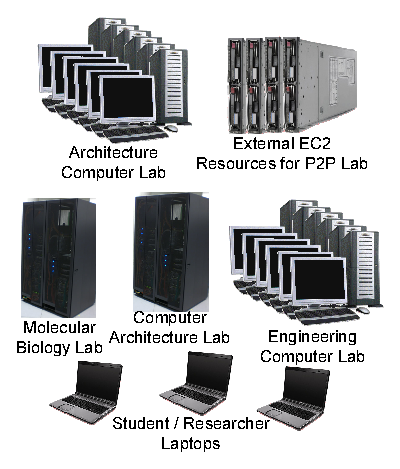
\epsfig{file=figs/unconnected.eps, width=3.25in}
\caption{A collection of various computing resources at a typical university}
\label{fig:unconnected}
\end{figure}

\subsection{Traditional Configuration of a Campus Grid}

A VPN must be used to connect the resources due to the lack of network symmetry
across the sites.  There exists a wealth of VPNs available~\cite{hamachi,
openvpn, tinc} and some explicitly for grids~\cite{violin, vine, vnet}.  For
simplicity sake, OpenVPN$^\registered$ was chosen due to the simplicity in its configuration.
In reality, OpenVPN$^\registered$ makes a poor choice because it is centralized, thus all
traffic between submitter and worker must traverse the VPNs server.  Whereas
others in the list are distributed and thus allow nodes to communicate
directly, but in order to do so, manual setup is required, a process, that
would overwhelm many novice grid deployers.  In all these cases, the VPN
requires that at least a single node have a public address, thus I had to make
a single concession in the design of this grid, that is, the OpenVPN$^\registered$ server
runs on a public node.

In order to connect to OpenVPN$^\registered$, it must know the server's address and have a
signed certificate.  While typically, most administrators would want a unique
private key for each machine joining the grid, in my case study and
evaluation, I avoided this process and used a common key, certificate pair.  In
doing so, there are potential dangers, for example, if any of the machines were
hijacked, the certificate would have to be revoked and all machines would be
rendered inoperable.  To create a properly secured environment, each resource
would have to generate or be provided a private key, a certificate request
submitted to the certificate authority, and a signed certificate provided to
the resource.

With the networking and security components in place, the next step is
configuring grid middleware.  Prior to deploying any resources, the manager
must be allocated and its IP address provider to other resources in the system.
Submission points are not a focus on this case study, though in general most
systems of this nature have a single shared submission site.  The challenges in
supporting multiple submission points in this environment include creating
certificates same as worker nodes,  requiring users to configure OpenVPN$^\registered$ and
Condor, and handling NFS mounts.  Whereas having a single submission point
creates more work for the system administrator as mentioned earlier.  Both
approaches have their associated costs and neither is trivial.  The evaluation
assumes a single user submitting from a single resource.

To address potential heterogeneity issues.  An administrator would need to
collaborate with others to ensure that all resources are running a common set
of tools and libraries.  Otherwise an application that works well on one
platform could cause a segmentation fault on another, through no fault of the
user, but rather due to library incompatibilities. 

To export this system into various clouds, an administrator starts by running
an instance that contains their desired Linux distribution and then installing
the grid utilities like Condor and OpenVPN$^\registered$.  Supporting individualization of
the resources is challenging.  The simplest approach is to store all the
configuration in that instance including the single private key, certificate
pair as well as the IP address of the manager node.  Alternatively, the
administrator could build an infrastructure that receives certificate requests
and returns a certificate.  The IP address of the manager node and of the
certificate request handler could be provided to the cloud via user data, a
feature common to most IaaS clouds that allows users to provide either text or
binary data that is available via a private URL inside a cloud instance.

\subsection{Grid Appliance in a Campus Grid}

All these configuration issues are exactly the reasons why ``Grid Appliance''
and its associated group Web interface are desirable for small and medium scale
grids.  The first component is deciding which web interface to use, public
(\url{www.grid-appliance.org}) or private hosted on their own resources.
Similarly, users can deploy their own P2P overlay or use the shared overlay.

The web interface enforces unique names for both the users and the groups.
Once the user has membership in the second tier of groups, they can download a
file that will be used to automatically configure their resources.  As
mentioned earlier, this handled obtaining a unique signed certificate,
connecting to the VPN, and discovering the manager in the grid.  Configuration
of the VPN and grid are handled seamlessly, the VPN automatically establishes
direct links with peers on demand and peers configure based upon information
available in the P2P overlay dynamically allowing for configuration changes.

Heterogeneity is a problem that will always exist if individuals are given
governance of their own resources.  Rather than fight that process, the ``Grid
Appliance'' approach is to provide a reference system and then include that
version and additional programs in the resource description exported by Condor.
Thus a user looking for a specific application, library, or computer
architecture can specify that in their job description.  Additionally, by means
of the transparent NFS mounts, users can easily compile their own applications
and libraries and export them to remote worker nodes.

Extending the ``Grid Appliance'' system into the clouds is easy.  The
similarity between a VM appliance and a cloud instance are striking.  The only
difference from the perspective of the ``Grid Appliance'' system is where to
check for configuration data.  Once a user has created a ``Grid Appliance'' in
a cloud, everyone else can reuse it and just supply their configuration data as
the user data during the instantiation of the instances.  As I describe in
Section~\ref{packaging}, creating ``Grid Appliance'' from scratch is a trivial
procedure.

As described in detail earlier, an administrator needs to install the necessary
software either by deploying VMMs and VM appliances or installing ``Grid
Appliance'' packages on Debian / Ubuntu systems.  Additionally, these systems
need to be packaged with the configuration files or floppy disk images.  At
which point, the systems will automatically configure and connect to the grid.
An administrator can verify this by monitoring Condor.  Additional resources
can be added seamlessly, likewise resources can be removed by shutting them off
without direct interaction with the ``Grid Appliance'' or manager node.

\subsection{Comparing the User Experience}

In the case of a traditional grid, most users will contact the administrator
and make a request for an account.  Upon receiving confirmation, the user will
have the ability to SSH into a submission site.  Their connectivity to the
system is instantaneous, their jobs will begin executing as soon as it is their
turn in the queue.  User's will most likely have access to a global NFS.  From
the user's perspective, the traditional approach is very easy and
straightforward.

With the ``Grid Appliance,'' a user will obtain an account at the web
interface, download a VM and a configuration file, and start the VM.  Upon
booting, the user will be able to submit and receive jobs.  To access the grid,
users can either SSH into the machine or use the consoles in the VM.  While
there is no single, global NFS, each user has their own unique NFS and must
make their job submission files contain their unique path.  For the most part,
the user's perspective of the ``Grid Appliance'' approach has much of the same
feel as the traditional approach.  Although users have additional features such
as accessing their files via Samba and having a portable environment for doing
their software development.

\subsection{Quantifying the Experience}

The evaluation of these environments focuses on the time taken to dynamically
allocate the resources, connect to the grid, and submit a simple job to all
resources in the grid.  In both systems, a single manager and submission node
were instantiated in separate VMs.  In the traditional setup, OpenVPN$^\registered$ is run
from the manager node.  Each component in the evaluation was run three times.
Between iterations, the submission node and the manager node were restarted to
clear any state.

The times measured include the time from when the last grid resource was
started to the time it reported to the manager node, Figure~\ref{fig:connect},
as well as the time required for the submit node to queue and run a 5 minute
job on all the connected workers, Figure~\ref{fig:run}.  The purpose of the
second test is to measure the time it takes for a submission site to queue a
task to all workers, connect to the workers, submit the job, and to receive the
results; thus a stress test on the VPN's ability to dynamically create links
and verifying all-to-all connectivity.  The tests were run on 50 resources
(virtual machines / cloud instances) in each environment and then on a grid
consisting of all 150 resources with 50 at each site.

\begin{figure}
\centering
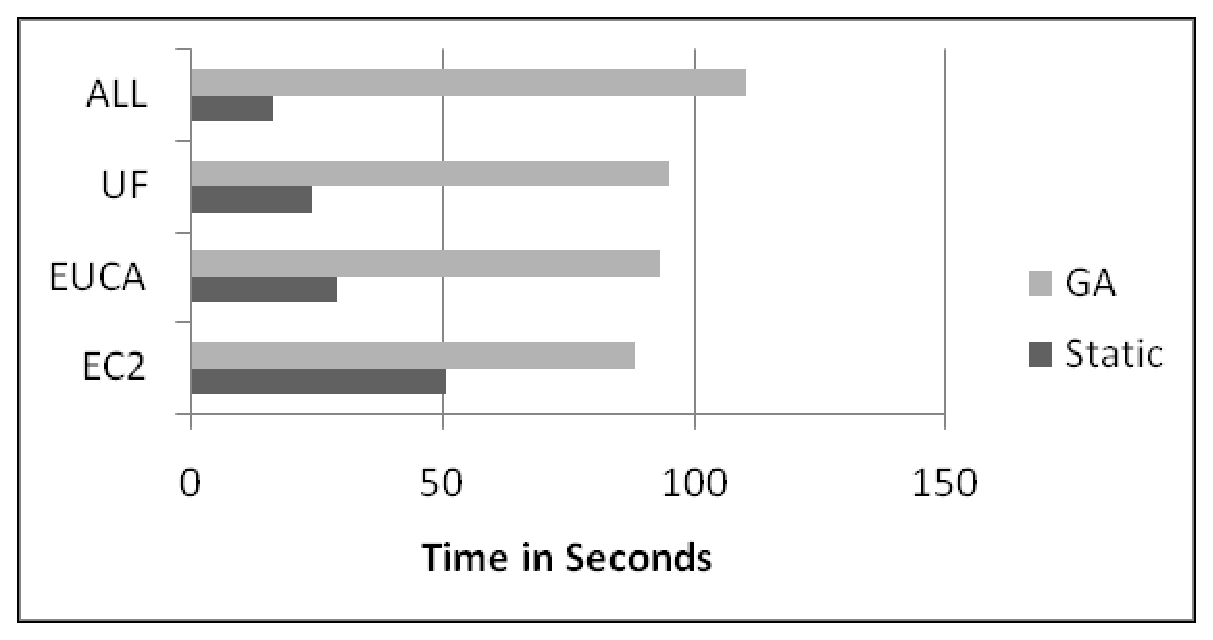
\epsfig{file=figs/connect.eps, width=4in}
\caption{Time to construct a grid}
\label{fig:connect}
\end{figure}

\begin{figure}
\centering
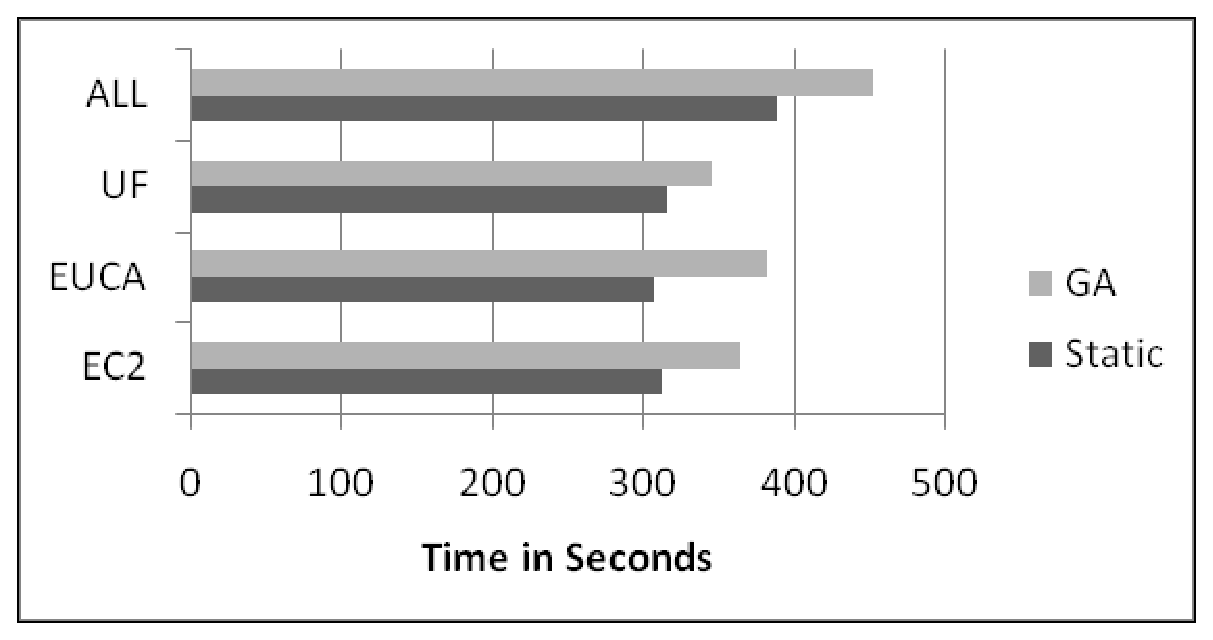
\epsfig{file=figs/run.eps, width=4in}
\caption{Time to run a job on a grid}
\label{fig:run}
\end{figure}

In the previous section, I qualified why the approach was easier than
configuring a grid by hand, though by doing so I introduce overheads related to
configuration and organization.  The evaluation verifies that these overheads
do not conflict with the utility of my approach.  Not only do resources within
a cluster install the VMs and connect to the grid quickly, the clouds do as
well.  While the results were similar, it should be noted that the time
required to configure the static approach was not taken into effect.  A process
that is difficult to measure and is largely reliant on the ability of the
administrator and the tools used.  Whereas the time for the ``Grid Appliance''
does include many of these components.

It should be stated that the evaluation only has a single submission node.  In
a system with multiple submitters, the OpenVPN$^\registered$ server could easily become a
bandwidth bottleneck in the system as all data must pass through it, which can
be avoided using IPOP.  Additionally, the current ``Grid Appliance'' relies on
polling with long delays, so as to not have negative effects on the system.
Either shrinking those times or moving to an event based system should
significantly improve the speed at which connectivity occurs.  

\section{Lessons Learned}
\label{lessons_learned}

This section highlights some the interesting developments and experiences, we
have had that do not fit the topics discussed so far.  

\subsection{Deployments}

A significant component of my experience stems from the computational grid
provided by Archer~\cite{archer}, an active grid deployed for computer
architecture research, which has been online for over 3 years.  Archer
currently spans six seed universities contributing over 600 CPUs as well as
contributions and activities from external users.  The Archer grid has been
accessed by hundreds of students and researchers from over a dozen institutions
submitting jobs totaling over 500,000 hours of job execution in the past two
years alone.

The Grid Appliance has also been utilized by groups at the Universities of
Florida, Clemson, Arkansas, and Northwestern Switzerland as a tool for teaching
grid computing.  Meanwhile the universities of Clemson and Purdue are using the
Grid Appliance's VPN (GroupVPN / IPOP) to create their own grid systems.  Over
time, there have been many private, small-scale systems using the shared system
available at \url{www.grid-appliance.org} with other groups constructing their
own independent systems.  Feedback from users through surveys have shown that
non-expert users are able to connect to the public Grid appliance pool in a
matter of minutes by simply downloading and booting a plug-and-play VM image
that is portable across VMware, VirtualBox, and KVM.

\subsection{Towards Unvirtualized Environments}
\label{packaging}

Because of the demands put on Archer in terms of avoiding the overheads of
virtualization and the perceived simplicity of managing physical resources as
opposed to virtual resources running on top of a physical resources, many users
have requested the ability to run Grid Appliances directly on their machine.
Unlike clouds with machine images such as AMIs (Amazon$^\registered$ Machine Image) or VM
appliances, physical machines images cannot be easily exported.  Most physical
OS installed on physical machines will need some some custom tailoring to
handle environment specific issues.

With this in mind, I moved away from stackable file systems and towards
creating repositories with installable packages, such as DEB or RPM.  The
implications of packages mean that users can easily produce ``Grid Appliances''
from installed systems or during system installation.  With the VPN router
mode, mentioned earlier, resources in a LAN can communicate directly with each
other rather than through the VPN.  That means if they are on a gigabit
network, they can full network speeds as opposed to being limited to 20\% of
that due to the VPN, overheads discussed in~\cite{sc09}.

\subsection{Advantages and Challenges of the Cloud}

I have had the experience of deploying the ``Grid Appliance'' on three
different cloud stacks:  Amazon$^\registered$'s EC2~\cite{ec2}, Future Grid's
Eucalyptus~\cite{eucalyptus}, and Future Grid's Nimbus~\cite{nimbus}.  All of
the systems, encountered so far, allow for data to be uploaded with each cloud
instance started.  The instance can then download the data from a static URL
only accessible from within the instance, for example, EC2 user data is
accessible at \url{http://169.254.169.254/latest/user-data}. A ``Grid
Appliance'' cloud instances can be configured via user-data, which is the same
configuration data used as the virtual and physical machines, albeit zip
compressed.  The ``Grid Appliance'' seeks the configuration data by first
checking for a physical floppy disk, then in specific directory
(\url{/opt/grid\_appliance/var/floppy.img}), followed by the EC2 / Eucalyptus
URL, and finally the Nimbus URL.  Upon finding a floppy and mounting it, the
system continues on with configuration.  Clouds have been also very useful for
debugging.  Though Amazon$^\registered$ is not free, with Future Grid, grid researchers now
have free access to both Eucalyptus and Nimbus clouds.  Many bugs can be
difficult to reproduce in small system tests or booting one system at a time.
By starting many instances simultaneously, I have been able to quickly
reproduce problems and isolate them, leading to timely resolutions, and
verification of those fixes.

Beyond the use of extending into clouds for on-demand resources, they are also
very convenient for debugging.  Doing so on Amazon$^\registered$ though is not free.
Fortunately, grid researchers now can have free access to Future Grid with both
Eucalyptus and Nimbus style clouds.  I did have to do some tinkering to get
these systems to work.  First, because the user data is binary data and the
communication exchange uses RPC, which may have difficulty handling binary
data, it must be converted to base64 before transferring and converted back
into binary data afterward.  EC2 handles this transparently, if using
command-line tools.  Unfortunately, Eucalyptus and Nimbus do not, even though
Eucalyptus is supposed to be compatible with EC2.

Furthermore, when starting an EC2 instance, networking is immediately
available, whereas with Eucalyptus and Nimbus, networking often times takes
more than 10 seconds after starting to be available. Thus a startup script must
be prepared for networking not to be ready and hence unable to immediately
download user data.  The best approach to deal with this in a distribution
independent manner is to wait until the primary Ethernet interface (eth0) has
an IP and then continuing.

\subsection{Stacked File Systems}

Configuring systems can be difficult, which makes it important to have the
ability to share the resulting system with others.  The approach of actually
creating packages can be overly complicated for novices.  To address this
concern, the original ``Grid Appliance'' supported a built-in mechanism to
create packages through a stackable file system using
copy-on-write~\cite{vtdc}.  In this environment, the VM used 3 disks: the
``Grid Appliance'' base image, the software stack configured by us; a module;
and a home disk.  In normal usage, both the base and module images are treated
as read-only file systems with all user changes to the system being recorded by
the home image, as depicted in Figure~\ref{fig:stackfs}.

\begin{figure}
\centering
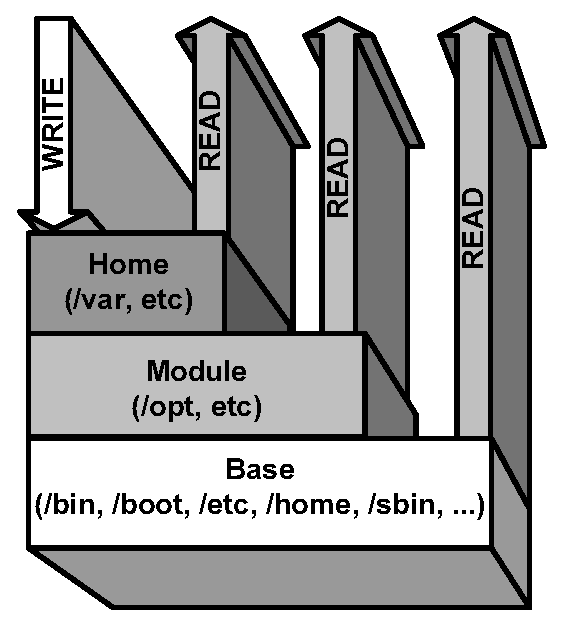
\epsfig{file=figs/stackfs.eps, width=2.5in}
\caption{Grid Appliance stackable file system}
\label{fig:stackfs}
\end{figure}

To upgrade the system, users replaced their current base image with a newer
one, while keeping their module and home disks.  While the purpose of the
module was to allow users to extend the configuration of the ``Grid
Appliance.''  To configure a module the system would be booted into developer
mode, an option during the boot phase, where only the base and module images
are included in the stacked file system.  Upon completing the changes, a user
would run a script that would clean the system and prepare it for sharing.  A
user could then share the resulting module image with others.

Issues with this approach made it unattractive to continue using.  First, there
exists no kernel level support for stackable file systems, I had to add
UnionFS~\cite{unionfs} to the kernel, adding the weight of maintaining a kernel
unto my shoulders.  While FUSE (filesystem in userspace) solutions exist, they
require modifications to the initial ram disk, which is reproduced
automatically during the installation of every new kernel, furthermore, our
experience with them suggests they are not well suited for production systems.
Additionally, the approach was not portable to clouds or physical resources.
So while I have deprecated the feature for now, I see it as a potential means
to easily develop packages like DEB and RPM.

\subsection{Priority in Owned Resources}

In Archer, seed universities should have priority on the resources at their
university.  Similarly, users should have priority on their contributions.
Otherwise, users will remove their resources from the grid, when they want
guaranteed access.  To support user and group based priorities, Condor has
mechanisms that can be enforced at the server that allow for arbitrary means to
specify user priority for a specific resource.  So the configuration specifies
that if the resource's user or group matches that of the submitter, the
priority is higher than otherwise.  This alone is not sufficient as malicious
users could easily tweak their user name or group to obtain priority on all
resources.  Thus whenever this check is made the user's identity in the
submission information is verified against their P2P VPN certificate.  Failed
matches are not scheduled and are stored in a log at the manager for the
administrator to deal with later.

To support this behavior, the following statements have been added to the
respective system's Condor configuration file:

\begin{tabbing}
Th\=e \=format for this configuration is as follows:\\
\> Job queue (server):\\
\> \> NEGOTIATOR\_PRE\_JOB\_RANK = 10 * (MY.RANK) \\
\> Worker:\\
\> \> GROUP\_RANK = TARGET.Group =?= MY.Group \\
\> \> USER\_RANK = TARGET.User =?= My.User \\
\> \> RANK = GROUP\_RANK $\vert\vert$ USER\_RANK \\
\>  Worker and Submitter:\\
\> \> Group = "Group's Name"\\
\> \> User = "User's Name"
\end{tabbing}

\subsection{Timing in Virtual Machines}

Certain applications, particularly license servers, are sensitive to time.
Because of the nature of grids, there exist possibilities of having
uncoordinated timing, such as improperly specifying the time zone or not using
a network time protocol (NTP) server With regards to VMs,
VMWare~\cite{vmware_timing} suggests synchronizing with the host's time and to
avoid using services like NTP, which may have adverse affects on timing inside
the virtual machine.  While NTP might have some strange behavior, relying on
host time may produce erratic jumps in time that some software cannot handle.
My experiences recommends the use of NTP to address these concerns, which has
resolved many issues with strange software behavior and frustration from users
when their jobs fail due to being unable to obtain a license due to a timing
mismatch.

\subsection{Selecting a VPN IP Address Range}

One challenge in deploying a VPN is ensuring that the address space does not
overlap with that over the environments where it will be used.  If there is
overlap, users will be unable to connect to the VPN.  Doing so will confuse the
network stack, as there will be two network interfaces connected to the same
address space but different networks.  A guaranteed, though not necessarily
practical solution is to run the resource on a VM NAT or a cluster NAT that
does not overlap the IP address space of the VPN.

Users of the ``Grid Appliance'' should not have to concern themselves with this
issues.  Prior work on the topic by Ala Rezmerita et al.~\cite{pvc} recommends
using the experimental address class E ranging between 240.0.0.0 -
255.255.255.254, unfortunately this requires Linux kernel modifications.  With
the amount of bugs and security fixes regularly pushed into the kernel,
maintaining a forked kernel requires a significant amount of time, duplicating
the work already being performed by the OS distribution maintainers.  This
would also limit the ability to easily deploy resources in physical and cloud
environments.  Additionally, users that wanted to multipurpose a physical
resource may not want to run a modified kernel, while in most cloud setups the
kernel choice is limited.

I have since moved towards using the 5.0.0.0 - 5.255.255.255 address range.
Like the class E address space it is unallocated, but it requires no changes to
any operating systems.  The only limitation is that some other VPNs also use
it, thus a user would not be able to run two VPNs on the same address space
concurrently.  This approach is much better than providing kernels or dealing
with network address overlaps.  Interestingly, even with this in place, we
still see some ``GroupVPNs''  using address ranges in normal private network
address ranges for the VPN, like 10.0.0.0 - 10.255.255.255 and 192.168.0.0 -
192.168.255.255.

\subsection{Administrator Backdoor}

While most administrators will agree that most problems that users encounter
are self-inflicted, there are times, when the system is at fault.  Debugging
systems faults in a decentralized system can be very tricky, since it is very
difficult to track down a resource in order to gain direct physical access.
Additionally, having a user bring their resource to an administrator may be
prohibitively complicated, as the user would need to relocate their ``Grid
Appliance'' instance and have network connectivity in order to connect to the
grid and show the problem to the administrator.  To address this and other
concerns that only appear after running the system for long periods of time, we
have supplied an administrator backdoor into all resources by installing our
public ssh key, though users are informed of this and are free to remove it for
privacy concerns.  In typical configurations, this approach might not be
feasible, but because the ``Grid Appliance'' ships with a decentralized VPN
supporting all-to-all connectivity, any resource connected to the VPN is
accessible for remote debugging by an administrator.  Most users involved are
extremely delighted with the process as it has an appearance that the system
``just works.''

\section{Related Work}
\label{related_work}

Existing work that falls under the general area of desktop grids/opportunistic
computing include Boinc~\cite{boinc}, BonjourGrid~\cite{bonjourgrid}, and
PVC~\cite{pvc}.  Boinc, used by many ``@home'' solutions, focuses on adding
execute nodes easy; however, job submission and management rely on
centralization and all tasks must use the Boinc APIs.  BonjourGrid removes the
need for centralization through the use of multicast resource discovery; the
need for which limits its applicability to local area networks.  PVC enables
distributed, wide-area systems with decentralized job submission and execution
through the use of VPNs, but relies on centralized VPN and resource management.

Each approach addresses a unique challenge in grid computing, but none
addresses the challenge presented as a whole: easily constructing distributed,
cross-domain grids.  Challenges that I consider in the design of my system
include allowing submission sites to exist any where without being confined to
complex configuration or highly available, centralized locations; the ability
to dynamically add and remove resources by starting and stopping a a resource;
and the sharing of common servers so that no group in the grid is dependent on
another.  I emphasize these points, while still retaining the ease of use of
Boinc, the connectivity of PVC, and the flexibility of BonjourGrid.  The end
result is a system similar to OurGrid~\cite{ourgrid}; however, OurGrid requires
manual configuration of the grid and networking amongst sites, administration
of users within a site, and limits network connectivity amongst resources,
whereas ``Grid Appliance'' transparently handles these issues with a P2P
overlay and VPN to handle network constraints and support network sandboxing
and a web interface to configure and manage the grid.

With regards to clouds, there exists contextualization~\cite{context}.  Users
construct an XML configuration file that describes how a cloud instance should
be configured and provide this to a broker.  During booting of a cloud
instance, it will contact a third-party contextualization broker to receive
this file and configure the system.  This approach has been leveraged to create
dynamic grids inside the Nimbus cloud~\cite{alien_grid}.  While this approach
can reproduce similar features of the ``Grid Appliance,'' such as creating
grids inside the cloud, there are challenges in addressing cloud bursting,
automated signing of certificates, and collaboration amongst disparate groups.
